\chapter{Bulk-Boundary Correspondence Rebuilt}
\label{ch:bbc-rebuilt}

\begin{chapterlead}
The bulk-boundary correspondence is one of the deepest principles in
topological physics: the number of protected edge states at an interface
is determined by bulk topological invariants computed far from the
boundary. In Hermitian photonic systems, this correspondence is exact
and robust (Chapter~\ref{ch:berry-maxwell}). In non-Hermitian systems,
it can fail: the non-Hermitian skin effect
(Chapter~\ref{ch:skin-effect}) invalidates the Bloch-band invariants on
which the conventional correspondence is built. This chapter shows how
the correspondence is \emph{rebuilt}: not by abandoning topology, but by
computing invariants on the generalized Brillouin zone that faithfully
reflects the open-boundary physics.
\end{chapterlead}


%% ================================================================
\section{Why the conventional correspondence fails}
\label{sec:bbc-failure}

\subsection{The Hermitian baseline}
\label{ssec:hermitian-baseline}

Recall the logic of the Hermitian bulk-boundary correspondence.
For a one-dimensional topological insulator---the prototypical Su--Schrieffer--Heeger (SSH) chain with alternating hopping amplitudes
$t_1$ and $t_2$---the Bloch Hamiltonian is
\begin{equation}
 H(k) = \begin{pmatrix} 0 & t_1 + t_2\,e^{-ik} \\
 t_1 + t_2\,e^{ik} & 0 \end{pmatrix}.
 \label{eq:ssh-bloch}
\end{equation}
The winding number of the off-diagonal element $h(k) = t_1 + t_2\,e^{-ik}$
around the origin in the complex plane is
\begin{equation}
 \wnum = \frac{1}{2\pi i}\oint_{\mathrm{BZ}}
 \frac{h'(k)}{h(k)}\;\dd k
 = \begin{cases} 1 & |t_1| < |t_2|, \\ 0 & |t_1| > |t_2|. \end{cases}
 \label{eq:ssh-winding}
\end{equation}
When $\wnum = 1$, a finite open chain has one zero-energy edge state at
each boundary. When $\wnum = 0$, there are no edge states. The
topological phase transition occurs at $|t_1| = |t_2|$, where the bulk
gap closes. This is the conventional bulk-boundary correspondence:
the \emph{bulk} winding number, computed from the \emph{periodic}
Bloch Hamiltonian, predicts the \emph{boundary} physics of an
\emph{open} chain.

The correspondence works because, in a Hermitian system, the PBC and
OBC spectra agree in the thermodynamic limit. The Bloch eigenstates
are extended plane waves that faithfully represent the bulk physics,
regardless of boundary conditions.

\subsection{The non-Hermitian SSH model}
\label{ssec:nh-ssh}

Now consider a non-Hermitian generalization of the SSH model~\cite{lin2023topological,kunst2018biorthogonal}. The
simplest version introduces asymmetric intra-cell hopping:
\begin{equation}
 H_{\mathrm{NH}}(k) = \begin{pmatrix} 0 & t_1 + \gamma/2 + t_2\,e^{-ik} \\
 t_1 - \gamma/2 + t_2\,e^{ik} & 0 \end{pmatrix},
 \label{eq:nh-ssh-bloch}
\end{equation}
where $\gamma$ is a non-Hermitian parameter that makes the hopping
asymmetric ($t_1 + \gamma/2$ from right to left, $t_1 - \gamma/2$
from left to right within the unit cell). The Bloch Hamiltonian is no
longer Hermitian: $H_{\mathrm{NH}}(k) \neq H_{\mathrm{NH}}^\dagger(k)$.

\subsection{The failure}
\label{ssec:bbc-problem}

The conventional winding number, computed from $h(k) = t_1 + \gamma/2
+ t_2\,e^{-ik}$, predicts a topological phase transition at
\begin{equation}
 |t_1 + \gamma/2| = |t_2|
 \qquad\text{(Bloch prediction)}.
 \label{eq:bloch-transition}
\end{equation}
However, exact diagonalization of the open chain reveals that the
topological zero modes appear and disappear at a \emph{different}
parameter value:
\begin{equation}
 t_1 = \pm\sqrt{t_2^2 + (\gamma/2)^2}
 \qquad\text{(true OBC transition)}.
 \label{eq:obc-transition}
\end{equation}
The Bloch winding number gives the \emph{wrong phase diagram}~\cite{shen2017topological,yao2018edge,yokomizo2019non}.

The root cause is the non-Hermitian skin effect
(Chapter~\ref{ch:skin-effect}). Under OBC, the bulk spectrum develops
an extensive set of exponentially localized skin states
(Figure~\ref{fig:skin-mode-localization}), and the PBC and OBC spectra
can be very different
(Figure~\ref{fig:skin-pbc-obc-spectra}). The Bloch Hamiltonian,
which assumes extended eigenstates on the unit circle $|\beta| = 1$,
does not describe the open-boundary physics.

\begin{booknote}[A spectacular failure]
The failure is not a small quantitative correction. For $\gamma = 0.8$,
$t_2 = 1$, the Bloch prediction places the phase boundary at
$t_1 = 0.6$, while the true OBC boundary is at $t_1 \approx 1.077$.
The entire topological phase diagram is qualitatively wrong---including
regions where the Bloch invariant predicts a trivial phase but topological
edge states exist, and vice versa.
\end{booknote}

\paragraph{Worked numerical comparison.}
To make this failure quantitative, take $t_2 = 1$, $\gamma = 0.8$
and vary $t_1$ through the transition region. At $t_1 = 0.7$:
\begin{itemize}
 \item \textbf{Bloch prediction}: $|t_1 + \gamma/2| = |0.7 + 0.4| = 1.1 > 1$,
 so $\wnum_{\text{Bloch}} = 0$ (trivial).
 \item \textbf{Non-Bloch prediction}: GBZ radius
 $r = \sqrt{(t_1 - \gamma/2)/(t_1 + \gamma/2)} = \sqrt{0.3/1.1} \approx 0.522$;
 $\wnum_{\text{GBZ}} = 1$ (topological).
 \item \textbf{OBC exact diagonalisation} ($L = 80$): two robust
 zero-energy modes exist, confirming the non-Bloch prediction.
\end{itemize}
At $t_1 = 1.2$, both predictions agree: $\wnum = 0$ and no edge states.
The discrepancy region $0.6 < t_1 < 1.077$ is entirely missed by the
Bloch invariant. This is not a perturbative correction but a qualitative
failure of the conventional theory.

\paragraph{The skin effect as the root cause.}
The failure traces directly to the skin effect
(Chapter~\ref{ch:skin-effect}). Under OBC, the eigenstates of
$H_{\mathrm{NH}}$ are not extended Bloch waves but exponentially
localised skin modes with spatial envelope $\sim r^n$, where
$r = |\beta_{\mathrm{GBZ}}| \neq 1$. The Bloch Hamiltonian assumes
$|\beta| = 1$ and therefore probes the wrong region of the complex
$\beta$ plane. The GBZ corrects this by replacing the unit circle
with the contour $|\beta| = r$ that matches the open-boundary
eigenstates.

Physically, the skin effect means that the bulk modes themselves
carry information about the boundary: their exponential envelope
`knows' which boundary they are localised toward. The Bloch
description, which by construction ignores boundaries, cannot capture
this information. The non-Bloch theory restores the correspondence
by building boundary awareness into the very definition of the
Brillouin zone.

Figure~\ref{fig:ch15-non-bloch-bbc} summarises the three ingredients of
the failure and its resolution for the non-Hermitian SSH model at
$t_2 = 1$, $\gamma = 0.8$.

\begin{figure}[t]
 \centering
 
\includegraphics[width=0.98\linewidth]{fig_f15_non_bloch_bbc.pdf}
 \caption{Failure of the Bloch bulk-boundary correspondence and its
 non-Bloch resolution for the non-Hermitian SSH model with $t_2 = 1$
 and $\gamma = 0.8$.
 (a)~One-parameter phase strip. The dashed blue line marks the
 Bloch/PBC phase boundary at $t_1 = 0.60$; the solid red line marks
 the true OBC/GBZ transition at $t_1 = 1.077$. The orange region
 between them is topologically nontrivial only on the generalised
 Brillouin zone---a qualitative failure of the conventional Bloch
 invariant. The black dot marks $t_1 = 0.7$, the parameter used in
 panels~(b) and~(c).
 (b)~Generalised Brillouin zone in the complex $\beta$ plane. The
 dashed grey circle is the ordinary BZ ($|\beta| = 1$); the solid
 red circle is the GBZ with $|\beta| = 0.522$, computed from the
 transfer-matrix eigenvalue condition.
 (c)~Normalised intensity envelopes of representative OBC zero modes on
 a logarithmic scale. Green and purple mark modes localised at the two
 terminations. The decay is exponential with
 skin length $\xi_{\mathrm{skin}} = -1/\ln|\beta_{\mathrm{GBZ}}|
 \approx 1.54$ unit cells. Curves are clipped below $10^{-6}$ for
 display.}
 \label{fig:ch15-non-bloch-bbc}
\end{figure}


%% ================================================================
\section{The non-Bloch bulk-boundary correspondence}
\label{sec:non-bloch-bbc}

The resolution, introduced by Yao and Wang, is to compute topological
invariants on the generalized Brillouin zone
(Section~\ref{sec:gbz})---the contour in the complex $\beta$ plane
that correctly describes the open-boundary eigenstates.

\subsection{Statement}
\label{ssec:non-bloch-statement}

For a one-dimensional non-Hermitian system with chiral symmetry, the
\emph{non-Bloch bulk-boundary correspondence}~\cite{yao2018edge,yokomizo2019non,yang2020non} states:
\begin{equation}
 \boxed{
 N_{\mathrm{zero\;modes\;per\;interface}} = |\wnum_{\mathrm{GBZ}}|,
 }
 \label{eq:non-bloch-bbc}
\end{equation}
where $\wnum_{\mathrm{GBZ}}$ is the winding number computed on the
GBZ~\eqref{eq:non-bloch-winding}. For a finite SSH chain with two
topological terminations, the total number of zero modes is therefore
twice this value. This invariant correctly predicts the topological zero
modes throughout the gapped parameter regime, including where the
conventional Bloch invariant gives the wrong answer.

\subsection{The GBZ for the non-Hermitian SSH model}
\label{ssec:gbz-ssh}

For the non-Hermitian SSH model~\eqref{eq:nh-ssh-bloch}, replacing
$e^{ik} \to \beta$ yields the characteristic equation
\begin{equation}
 (t_1 + \gamma/2 + t_2\,\beta^{-1})(t_1 - \gamma/2 + t_2\,\beta) = E^2.
 \label{eq:nh-ssh-char}
\end{equation}
At $E = 0$ (the gap-closing energy for chiral-symmetric systems), this
gives four solutions for $\beta$. Ordering them by modulus,
$|\beta_1| \le |\beta_2| \le |\beta_3| \le |\beta_4|$, the GBZ
condition~\eqref{eq:gbz-condition} requires $|\beta_2| = |\beta_3|$.

For this model, the GBZ is a circle of radius
\begin{equation}
  |\beta_{\mathrm{GBZ}}| = r
  = \sqrt{\frac{|t_1 - \gamma/2|}{|t_1 + \gamma/2|}}.
  \label{eq:gbz-radius-ssh}
\end{equation}
The final equality assumes the positive real parameter regime used in the
example.  The intercell hopping $t_2$ sets the overall frequency
scale for this symmetric intercell choice and therefore does not affect
the GBZ radius.  In the Hermitian limit $\gamma=0$, the radius becomes
$r=1$, so the GBZ reduces continuously to the ordinary Brillouin zone.
The GBZ-based winding number is computed by evaluating $h(\beta)$ on this
deformed contour rather than on the unit circle.

\subsection{Derivation of the non-Bloch BBC}
\label{ssec:bbc-derivation}

The key idea is that the open-boundary eigenstates at zero energy are
determined by the transfer-matrix eigenvalues at $E = 0$. For a chain
of $L$ unit cells, a zero-energy eigenstate must satisfy the boundary
conditions at both the left and right ends. Writing the spatial
dependence as a sum of the four transfer-matrix solutions
$\psi_n \sim \sum_j c_j\,\beta_j^n$, normalizability imposes constraints
from both boundaries.

From the left boundary, the coefficients of the solutions that grow
toward the left ($|\beta_j| > 1$ when viewed from the left end) must
vanish; otherwise $|\psi_n|$ would diverge as $n \to \infty$.
Similarly, from the right boundary, the coefficients of the solutions
that grow toward the right ($|\beta_j| < 1$ when viewed from the right
end) must vanish from the right-end perspective. For a system with
$2n$ transfer-matrix eigenvalues ordered by modulus
$|\beta_1| \le |\beta_2| \le \cdots \le |\beta_{2n}|$, a normalizable
zero mode exists precisely when the boundary conditions can be
simultaneously satisfied---that is, when exactly $n$ eigenvalues lie
inside the GBZ contour and $n$ lie outside.

The GBZ contour is defined by the condition $|\beta_n| = |\beta_{n+1}|$:
the two ``middle'' eigenvalues must have equal modulus. This is
because the zero mode at the interface between the inside and outside
groups must change character precisely at the GBZ radius. When this
condition holds, the transfer-matrix problem has a self-consistent
solution that is normalizable from both ends simultaneously.

As parameters are varied, a zero mode appears or disappears when a
$\beta_j$ \emph{crosses the GBZ contour}---not when it crosses the unit
circle. The winding number computed on the GBZ counts how many times
this crossing has occurred, and therefore correctly predicts the number
of topological zero modes.

\paragraph{Physical interpretation of the GBZ radius.}
The GBZ radius $r = |\beta_{\mathrm{GBZ}}|$ has a direct physical
meaning: it determines the \emph{skin localisation length}
\begin{equation}
 \xi_{\mathrm{skin}} = \frac{-1}{\ln r},
 \label{eq:skin-length-from-gbz}
\end{equation}
measured in unit cells. When $r < 1$, the bulk skin states are
exponentially localised toward the left boundary with decay length
$\xi_{\mathrm{skin}}$; when $r > 1$, they localise toward the right.
In the Hermitian limit $r \to 1$, $\xi_{\mathrm{skin}} \to \infty$ and
the bulk modes become extended Bloch waves.

For the non-Hermitian SSH model with $t_2 = 1$ and $\gamma = 0.8$, the
GBZ radius is $r = 0.522$ (Figure~\ref{fig:ch15-non-bloch-bbc}b),
giving a skin length $\xi_{\mathrm{skin}} = 1/|\ln 0.522| \approx
1.54$ unit cells---an extremely strong localisation. This quantitative
prediction can be tested directly by measuring the spatial decay of the
field envelope in a finite photonic lattice, as demonstrated in
microwave waveguide networks and acoustic metamaterials.

\paragraph{GBZ for general two-band models.}
The GBZ construction generalises straightforwardly to any two-band
non-Hermitian model with nearest-neighbour coupling. The Bloch
Hamiltonian takes the form
$H(\beta) = \sum_j d_j(\beta)\,\sigma_j$ where
$d_j(\beta) = d_j^{(0)} + d_j^{(+)}\beta + d_j^{(-)}\beta^{-1}$.
The characteristic equation $\det(E - H(\beta)) = 0$ is a polynomial
in $\beta$ (typically quartic for two-band models), and the GBZ is
the contour in the complex $\beta$ plane on which the middle pair
of roots has equal modulus. For models with only one asymmetric
hopping parameter (such as the Hatano--Nelson model), the GBZ is a
circle and the calculation reduces to finding a single radius $r$.
For models with multiple asymmetric parameters, the GBZ can be a
non-circular closed curve, and the winding number must be computed
numerically by discretising the GBZ contour and tracking the phase
of $\det H(\beta)$. The algorithms for this computation are
discussed in Chapter~\ref{ch:numerics}.

\begin{remark}
The derivation shows why the \emph{shape} of the GBZ matters, not just
its existence. For models where the GBZ is not a circle (e.g.,
multi-band or long-range hopping models), the contour can be
self-intersecting or multi-sheeted, and the winding number must be
computed on the full geometric GBZ rather than a simple circle.
\end{remark}


%% ================================================================
\section{Example: non-Hermitian SSH phase diagram}
\label{sec:nh-ssh-example}

To make the non-Bloch BBC concrete, consider the non-Hermitian SSH
model with $t_2 = 1$ and $\gamma = 0.8$.

\subsection{Bloch versus non-Bloch phase boundaries}
\label{ssec:phase-boundaries}

The conventional Bloch winding number predicts a topological phase
transition at $|t_1 + 0.4| = 1$, i.e., $t_1 = 0.6$ or $t_1 = -1.4$.
The non-Bloch winding number, computed on the GBZ, predicts a
transition at $t_1 = \sqrt{1 + 0.16} \approx 1.077$. These are
quantitatively different---the Bloch prediction misplaces the phase
boundary by nearly a factor of two.

\subsection{OBC spectrum and edge states}
\label{ssec:obc-edge}

Exact diagonalization of an open chain of $L = 60$ unit cells confirms
the non-Bloch prediction. For $t_1 = 0.8$ (between the Bloch and
non-Bloch boundaries), the Bloch invariant gives $\wnum = 0$ (trivial),
but the OBC spectrum shows two robust zero-energy edge states. For
$t_1 = 1.2$ (above the non-Bloch boundary), the edge states vanish.

This example demonstrates that the non-Bloch BBC is essential for
predicting the topological phase diagram of non-Hermitian systems with
the skin effect.


%% ================================================================
\section{Biorthogonal bulk-boundary correspondence}
\label{sec:biorthogonal-bbc}

An alternative approach to rebuilding the bulk-boundary correspondence
uses the \emph{biorthogonal polarization}---a non-Hermitian
generalization of the electric polarization or Zak phase.

\subsection{Biorthogonal polarization}
\label{ssec:biorthogonal-pol}

In a Hermitian system, the bulk polarization is defined as the integral
of the Berry connection over the Brillouin zone. In a non-Hermitian
system, the biorthogonal polarization uses the left and right
eigenvectors:
\begin{equation}
 P^{\mathrm{bi}} = \frac{1}{2\pi}\oint_{\BZ}
 i\,\frac{\langle u_k^{\mathrm{L}}|\partial_k|u_k^{\mathrm{R}}\rangle}
 {\langle u_k^{\mathrm{L}}|u_k^{\mathrm{R}}\rangle}\;\dd k.
 \label{eq:biorthogonal-pol}
\end{equation}
This quantity is quantized (modulo integers) by chiral symmetry and
predicts the existence of edge states in the biorthogonal
framework.

\begin{figure}[t]
 \centering
 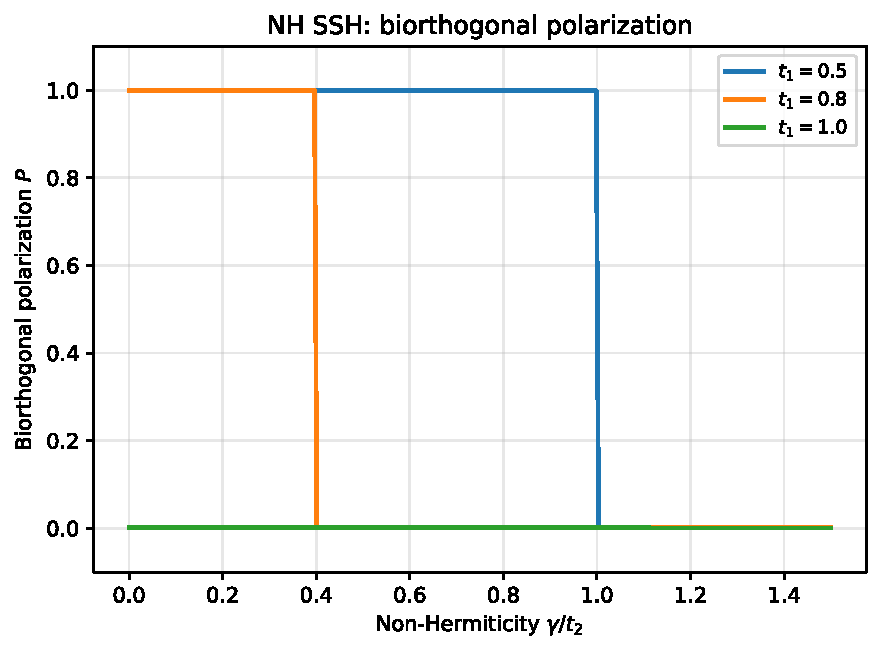
\includegraphics[width=0.6\linewidth]{figures/fig_f15_biorthogonal_pol.pdf}
 \caption{Biorthogonal polarization diagnostic as a function of
 non-Hermiticity $\gamma/t_2$ for different intracell hoppings $t_1$ in
 the NH SSH model. The plotted convention uses values $0$ and $1$ for
 the two quantized sectors; in the usual polarization convention these
 correspond to $P=0$ and $P=1/2$ modulo one. The jump marks the
 non-Hermitian topological transition in this biorthogonal diagnostic.
 Chiral symmetry pins the value to a quantized sector away from gap
 closings.}
 \label{fig:biorthogonal-pol}
\end{figure}

\subsection{Physical interpretation}
\label{ssec:biorthogonal-interpretation}

The biorthogonal polarization has a direct physical interpretation.
In a Hermitian system, the bulk polarization measures the displacement
of charge (or field energy) within the unit cell. In a non-Hermitian
system, $P^{\mathrm{bi}}$ measures the displacement of the
\emph{biorthogonal} charge density $\rho^{\mathrm{bi}}(x) =
\langle\psi^{\mathrm{L}}(x)|\psi^{\mathrm{R}}(x)\rangle$, which
can be complex. The quantization of $P^{\mathrm{bi}}$ reflects the
fact that a half-integer displacement of the biorthogonal charge
(modulo one) signals a topological phase with boundary-localized
modes.

\paragraph{Example: biorthogonal polarisation of the NH SSH model.}
For the non-Hermitian SSH model~\eqref{eq:nh-ssh-bloch} with
$t_1 = 0.5$, $t_2 = 1$, $\gamma = 0.6$, the right eigenvector of the
lower band is
$|u_k^{\mathrm{R}}\rangle = (1,\; -E(k)/h(k))^\transpose$ (up to
normalisation and branch convention), where $E(k) = \sqrt{h(k)\tilde{h}(k)}$,
$h(k) = t_1 + \gamma/2 + t_2 e^{-ik}$, and
$\tilde{h}(k) = t_1 - \gamma/2 + t_2 e^{ik}$. The left eigenvector is
obtained from the transpose/adjoint eigenproblem with the corresponding
left-right normalization. Numerical integration of the biorthogonal
connection, or equivalently the non-Bloch version evaluated on the GBZ
when skin modes are present, gives the quantized topological sector.
For this parameter set the polarization is in the topological sector
($P=1/2$ modulo one in the usual convention). When $t_1$ is increased
past the non-Bloch transition
($t_1 = \sqrt{t_2^2 + (\gamma/2)^2} = \sqrt{1.09} \approx 1.044$),
the non-Bloch/biorthogonal diagnostic jumps discontinuously to the trivial sector
(trivial), in agreement with the non-Bloch winding number. The jump
is sharp---not a smooth crossover---because $P^{\mathrm{bi}}$ is
quantised by chiral symmetry.

This confirms that the biorthogonal polarisation and the non-Bloch
winding number are two faces of the same topological invariant: they
detect the same phase transitions and predict the same edge states,
but provide different physical pictures---one based on GBZ deformation,
the other on biorthogonal charge displacement.

\subsection{Connection to QNM inner products}
\label{ssec:biorthogonal-qnm}

The biorthogonal polarization~\eqref{eq:biorthogonal-pol} is closely~\cite{kunst2018biorthogonal}
related to the unconjugated inner product used for quasinormal modes
(Section~\ref{sec:qnm-adjoint}). In both cases, the key mathematical
structure is the pairing between left (adjoint) and right eigenstates.
For a photonic system described by the Maxwell operator
$\hat{\Theta}$, the biorthogonal Berry connection becomes
\begin{equation}
 A_k^{\mathrm{bi}} = i\,
 \frac{\langle\tilde{\EE}_k^{\mathrm{L}}|
 \partial_k|\tilde{\EE}_k^{\mathrm{R}}\rangle_{\varepsilon}}
 {\langle\tilde{\EE}_k^{\mathrm{L}}|
 \tilde{\EE}_k^{\mathrm{R}}\rangle_{\varepsilon}},
 \label{eq:biorthogonal-berry-bbc}
\end{equation}
where $\langle\cdot|\cdot\rangle_\varepsilon$ is the unconjugated
inner product weighted by the permittivity tensor. This connects the
topological classification of non-Hermitian photonic bands directly to
the QNM formalism of Chapter~\ref{ch:qnm}.

\subsection{Relation to the non-Bloch approach}
\label{ssec:bbc-comparison}

The biorthogonal and non-Bloch approaches give consistent predictions
when the inner product and integration contour are chosen for the same
boundary problem, but they emphasize complementary physical insights:
\begin{itemize}
 \item The \textbf{non-Bloch approach} directly accounts for the
 skin effect by deforming the integration contour; it gives the
 correct phase diagram and the correct localization properties
 of edge states.
 \item The \textbf{biorthogonal approach} replaces the inner product
 with a left-right one and is more closely connected to the formalism
 of Chapter~\ref{ch:qnm} and the adjoint modes of the Maxwell operator.
 When the skin effect is present, its bulk version must be combined
 with the non-Bloch contour or with open-boundary biorthogonal states.
 \item For systems \emph{without} the skin effect (e.g., systems with
 reciprocity or additional symmetries that prevent the spectral
 loop from winding), the biorthogonal approach may be the only
 relevant non-Hermitian correction.
 \item For systems \emph{with} the skin effect, both approaches are
 needed for a complete picture: the non-Bloch approach gives the
 correct phase diagram, and the biorthogonal approach clarifies
 the physical meaning of the topological invariant.
\end{itemize}


%% ================================================================
\section{Higher-dimensional correspondence}
\label{sec:bbc-higher-d}

In two and higher dimensions, rebuilding the bulk-boundary
correspondence requires both non-Bloch band theory and the spectral-area
diagnostics discussed in Chapter~\ref{ch:point-gap}~\cite{zhang2022universal}.

\subsection{Non-Bloch Chern insulator}
\label{ssec:non-bloch-chern-insulator}

For a two-dimensional non-Hermitian Chern insulator, the non-Bloch Chern
number (Section~\ref{ssec:non-bloch-chern}) correctly predicts the
number of chiral edge modes, which can differ from the prediction of the
conventional Chern number when the skin effect is present.

The construction is conceptually straightforward: the two-dimensional
GBZ is the product of two one-dimensional GBZ contours (one for each
reciprocal direction), and the non-Bloch Chern number is the integral
of the Berry curvature over this deformed torus. In practice, computing
the two-dimensional GBZ is more involved because the GBZ contour in
each direction can depend on the momentum in the other direction.

\subsection{Corner modes and higher-order topology}
\label{ssec:corner-modes}

In certain two-dimensional systems, an extensive set of eigenstates can
be localized at
\emph{corners} rather than edges---the corner-skin effect
(Section~\ref{sec:skin-2d}). The relevant topological invariant is a
second-order non-Bloch invariant, defined by a nested GBZ construction:
first compute the GBZ in one direction at fixed momentum in the other,
then compute a one-dimensional topological invariant on the resulting
edge theory.

The corner modes predicted by this construction are exponentially
localized at zero, one, or two corners of a rectangular sample, depending
on the non-Bloch invariant and the orientation of the skin effect.

\subsection{Geometry dependence}
\label{ssec:geometry-dependence}

The geometry-dependent skin effect (Section~\ref{sec:skin-2d}) means that
the bulk-boundary correspondence itself can depend on the sample shape.
For example, a hexagonal sample may exhibit edge states on some edges but
not others, depending on the orientation of the non-reciprocal hopping.
This shape dependence has no Hermitian counterpart and requires a
boundary-condition-aware formulation of the topological invariant.


%% ================================================================
\section{Photonic implications}
\label{sec:bbc-photonic}

For photonic systems described by the Maxwell equations, the rebuilt
bulk-boundary correspondence has several practical implications.

\subsection{Photonic GBZ construction}
\label{ssec:photonic-gbz}

For a 1D non-Hermitian photonic system with effective nonreciprocal or
non-unimodular evolution, the GBZ can be constructed directly from the
Maxwell transfer matrix without passing through a tight-binding
approximation. The procedure is:
\begin{enumerate}
 \item Compute the unit-cell transfer matrix $M(\omega)$ at each
 complex frequency $\omega$ using the complex-$n_j$ layer
 propagation matrices of Chapter~\ref{ch:point-gap}.
 \item Find the eigenvalues $\beta_{1,2}(\omega)$ of $M(\omega)$.
 \item The GBZ is the corresponding contour in the complex $\beta$
 plane where the middle transfer-matrix roots have equal modulus; for a
 two-root problem this condition is $|\beta_1(\omega)|=|\beta_2(\omega)|$.
 \item On this contour, evaluate the photonic topological invariant
 (winding number or biorthogonal polarisation).
\end{enumerate}
For a reciprocal isotropic layer stack described by the usual
two-component field vector, the unit-cell transfer matrix is unimodular
even with material loss or gain. Then $\beta_1\beta_2=1$, and the
condition $|\beta_1|=|\beta_2|$ reduces to $|\beta_1|=|\beta_2|=1$.
Complex permittivity can still produce complex bands and evanescent
solutions, but it does not by itself generate a Hatano--Nelson-type GBZ
deformation. A genuine photonic non-Bloch correction requires an
effective evolution that breaks this cancellation, for example through
magneto-optical bias, temporal modulation, cascaded reservoirs, or a
multi-port network after unobserved channels are eliminated.

\paragraph{Connection to the photonic transfer-matrix formalism.}
The photonic GBZ construction links directly to the transfer-matrix
band theory of Chapter~\ref{ch:periodicity}: the Bloch condition
$\cos(Ka)=\xi(\omega)$ is replaced, in the effective nonreciprocal
problem, by the middle-root condition defining the GBZ. Instead of
solving only for real $K$ on the unit circle, one solves for the complex
$K$ values that reproduce the open-boundary spectrum. This makes the
non-Bloch theory of photonic topological phases accessible to the same
transfer-matrix and scattering tools used routinely in multilayer and
coupled-resonator design, provided the effective model includes the
channels responsible for directional gain or hopping.

\subsection{Design of robust edge channels}
\label{ssec:robust-edge}

In a non-Hermitian photonic crystal, edge channels designed using
conventional (Bloch) topological invariants may not appear or may appear
at unexpected parameter values. The non-Bloch approach provides a
concrete design rule: compute the GBZ for the target structure, evaluate
the topological invariant on the GBZ, and verify the edge-state
prediction against finite-structure simulations. This ensures that
the designed edge states are robust and correctly placed.

The practical difficulty is that computing the photonic GBZ requires
solving the Maxwell transfer matrix at complex frequencies and complex
wave vectors---a task that goes beyond standard photonic band-structure
calculations but is within the reach of the numerical methods of
Chapter~\ref{ch:numerics}.

\subsection{Directional amplification}
\label{ssec:directional-amp}

The skin effect combined with edge-state topology enables
\emph{topological amplifiers}: devices where light injected at one
boundary is amplified while propagating along an edge channel,
with directionality set by the non-Bloch topology and by the engineered
gain profile. The amplification can scale exponentially over the useful
device length, but in a physical photonic structure it is limited by
saturation, radiation loss, and disorder-induced mode mixing rather than
being absolutely immune to backscattering.

\subsection{Spectral engineering}
\label{ssec:spectral-engineering}

The dramatic difference between PBC and OBC spectra in non-Hermitian
photonic crystals can be exploited for spectral engineering. By
choosing boundary conditions (periodic, open, or mixed), the same
photonic structure can exhibit qualitatively different spectral
properties. For example, a ring resonator (PBC) and a terminated
waveguide array (OBC) made from the same non-Hermitian photonic crystal
will have different resonance frequencies, different mode spacings, and
different field distributions.

\subsection{Experimental signatures}
\label{ssec:experimental-signatures}

The non-Bloch BBC makes testable predictions for photonic experiments:
\begin{enumerate}
 \item \textbf{Edge-state presence:} the appearance or disappearance
 of edge modes as a function of gain/loss or coupling asymmetry
 should follow the non-Bloch phase boundary, not the Bloch one.
 \item \textbf{Spectral collapse:} the PBC-to-OBC spectral change
 (Figure~\ref{fig:skin-pbc-obc-spectra}) is a direct observable
 in coupled-resonator experiments where periodic or open boundary
 conditions can be implemented.
 \item \textbf{GBZ deformation:} the GBZ radius
 (Figure~\ref{fig:gbz-circle}) manifests as the exponential
 envelope of the skin modes, which can be measured from the
 spatial intensity profile.
\end{enumerate}

\paragraph{Edge-state penetration depth.}
In the non-Hermitian SSH model used in Fig.~\ref{fig:edge-localisation},
$t_1 = 0.6$, $t_2 = 1.0$, and the nonreciprocal hopping parameter is
$\delta = 0.3$.  The right zero mode on sublattice A obeys the open-chain
recursion
\begin{equation}
  (t_1-\delta)A_n + (t_2+\delta)A_{n+1}=0,
  \qquad
  \frac{|A_{n+1}|}{|A_n|}=\left|\frac{t_1-\delta}{t_2+\delta}\right|,
  \label{eq:edge-recursion}
\end{equation}
so the amplitude penetration depth is
\begin{equation}
  \xi_{\mathrm{edge}}
  = \frac{1}{\ln\left|(t_2+\delta)/(t_1-\delta)\right|}
  = \frac{1}{\ln(1.3/0.3)}
  \approx 0.68\;\text{cells}.
  \label{eq:edge-penetration}
\end{equation}
The Hermitian estimate obtained by setting $\delta=0$ is
$\xi_{\mathrm{Herm}}=1/\ln|t_2/t_1|\approx1.96$ cells, but that estimate
ignores the nonreciprocal intracell/intercell imbalance.  The non-Bloch
calculation and the direct OBC eigenvector therefore agree: the edge mode
is much more tightly confined than the Hermitian SSH formula would
suggest.  The exponential envelope $\propto e^{-x/\xi_{\mathrm{edge}}}$
has been confirmed experimentally in coupled-resonator arrays at both
microwave and optical frequencies, where the spatial intensity profile of
the edge mode can be measured site by site.

\begin{figure}[t]
 \centering
 
\includegraphics[width=0.82\linewidth]{fig_f15_edge_localisation.pdf}
  \caption{Sublattice-A amplitudes of the zero-energy edge state in
  the non-Hermitian SSH model ($t_1 = 0.6$, $t_2 = 1.0$,
  $\delta = 0.3$) under open boundary conditions, normalized to the
  boundary site. Red dashed: exponential fit to the first eight sites
  gives $\xi_{\mathrm{fit}} \approx 0.68$ cells, in agreement with the
  nonreciprocal zero-mode recursion~\eqref{eq:edge-recursion}. Green
  dotted: the Hermitian estimate
  $\xi_{\mathrm{Herm}} = 1/\ln(t_2/t_1) \approx 1.96$ cells, which
  ignores the hopping asymmetry $\delta$. The discrepancy is therefore
  not a plotting artifact but the edge-state analogue of the non-Bloch
  correction: the correct decay length follows from the open-boundary
  recursion or, equivalently, from the generalized Brillouin zone.}
 \label{fig:edge-localisation}
\end{figure}

\begin{figure}[t]
 \centering
 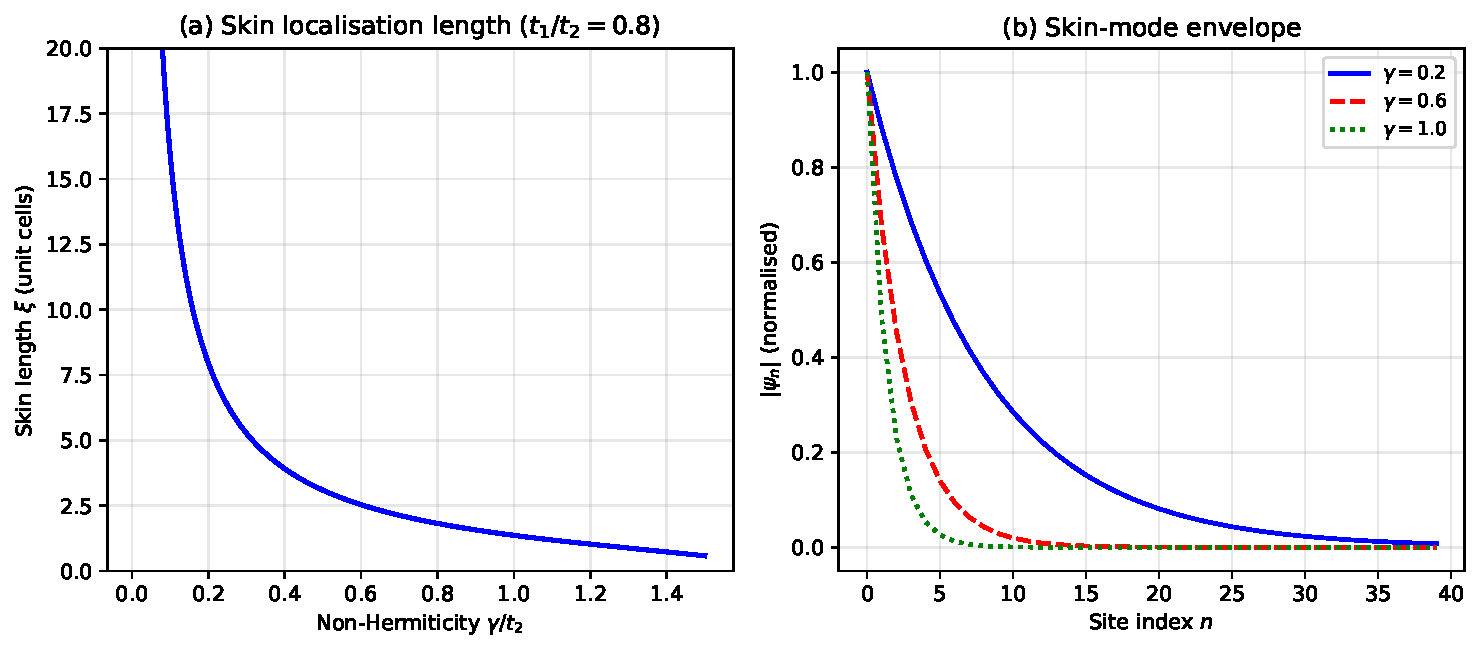
\includegraphics[width=0.85\linewidth]{figures/fig_f15_edge_penetration.pdf}
 \caption{Skin-effect localisation in the NH SSH model
 ($t_1/t_2 = 0.8$).
 (a)~Skin localisation length $\xi$ as a function of the
 non-Hermiticity parameter $\gamma$: $\xi$ diverges as
 $\gamma \to 0$ (Hermitian limit, where all bulk modes become
 extended) and decreases monotonically with increasing asymmetry.
 (b)~Skin-mode envelope $|\psi_n|$ for three values of $\gamma$,
 showing progressively stronger localisation toward one boundary
 as the non-Hermiticity grows.}
 \label{fig:edge-penetration}
\end{figure}

\paragraph{Experimental verification at optical frequencies.}
Photonic and microwave coupled-resonator experiments can test the
non-Bloch BBC by comparing spectra under ring-closed and ring-terminated
boundary conditions. The key checks are qualitative and quantitative:
the measured phase boundary should follow the GBZ prediction, and the
observed edge-mode localisation length should match the open-boundary
recursion or Eq.~\eqref{eq:edge-penetration} within fabrication
tolerance. Such measurements would test the non-Bloch correction to the
topological properties of non-Hermitian photonic systems.

\begin{takeaway}[The bulk-boundary correspondence survives]
The bulk-boundary correspondence is not destroyed by non-Hermiticity---it
is transformed. In its rebuilt form, it connects topological invariants
computed on the generalized Brillouin zone (or using biorthogonal inner
products) to the edge-state structure of open non-Hermitian systems.
The correspondence remains exact and robust, but it requires the non-Bloch
theory of Chapter~\ref{ch:skin-effect}: the unit circle is no longer the
correct Brillouin zone, the Bloch winding number is no longer the correct
invariant, and the Bloch phase diagram is no longer the correct map.
Once these replacements are made, the deep connection between bulk
topology and boundary physics is fully restored.
\end{takeaway}
